\documentclass{experimentreport}

\input{listing_style.tex}

%========================
% 图表支持
%========================
\usepackage{amsmath}
\usepackage{graphicx}
\usepackage{booktabs}
\usepackage{float}
\usepackage{caption}
\captionsetup{font=small,labelfont=bf,skip=4pt}
\graphicspath{{../results/figures/}}

%========================
% 基本信息
%========================

\setcoursename{基础软件开发技术实践}
\setreportname{智能软件工程实验报告}

\setexperimenttitle{实验四：基于大语言模型与 Prompt Engineering 的代码审查}

\setstudentname{\hintholder{王皓}}
\setdepartment{\hintholder{计算学部}}
\setstudentid{\hintholder{2023111825}}

\setcourseteacher{刘佳琨}
\setinstructor{刘佳琨}

\setlablocation{\hintholder{格物213}}
\setlabtime{    \hintholder{2026年7月2日}}

\begin{document}

%========================
% 自动生成封面
%========================

\makereporthead

%========================
% 实验目的
%========================

\experimentpurpose{

完成本实验后，学生应能够：

\begin{enumerate}
  \item 理解大语言模型在代码审查任务中的应用原理。
  \item 掌握Prompt Engineering的基本思想与设计方法。
  \item 理解不同代码上下文对大语言模型性能的影响。
  \item 能够利用大语言模型完成Merge Prediction任务。
  \item 能够利用大语言模型自动生成代码审查意见。
  \item 能够分析不同Prompt设计和上下文信息对代码审查结果的影响。
\end{enumerate}

}

%========================
% 实验内容
%========================

\experimentcontent{

本实验在整门课程中的定位是 \textbf{代码审查任务的大语言模型方案}：不训练任何模型，只通过设计输入来完成合并预测与审查意见生成，为实验二（传统机器学习）、实验三（深度学习）提供 LLM 侧的性能对照，并共同构成 ML $\rightarrow$ DL $\rightarrow$ LLM 的完整对比链条。这一范式的价值不在于取得最高精度，而在于\textbf{免训练、上下文可塑、结果可解释}——模型能力被视作固定常量，唯一可优化的自由度是喂给模型什么，因此本实验的核心问题是：在不训练模型的前提下，代码上下文与提示策略这两个维度各自及交互地在多大程度上决定审查质量。本部分先给出整体技术路线，再依次说明各环节的详细设计与实现，最后说明为支撑结果分析而设置的对照与下游分析。

\subsection*{2.1 总体技术路线}

本实验并列复用实验一清洗得到的关系型数据集与实验二固定的 train/test 划分，将冻结模型、优化输入的思路实例化为一条自包含、可复现的流水线：\textbf{分层抽样 $\rightarrow$ 多粒度上下文构建 $\rightarrow$ Prompt 模板注入 $\rightarrow$ 在线 LLM 调用（带重试、计时与缓存）$\rightarrow$ 结构化解析落盘 $\rightarrow$ 指标评估与跨范式对比}。贯穿全流程的方法论主线是\textbf{把输入拆成两个正交维度}——4 种上下文与 4 种 Prompt——做全因子实验，从而既能观察每个维度的边际效应，也能观察二者的交互。为保证结果可复现，所有随机性（抽样、few-shot 选例）均固定随机种子，所有网络调用均以语义 key 落盘缓存，任何中断或重跑都不会重复付费。整条流水线共产生 $\text{2 任务}\times\text{4 上下文}\times\text{4 Prompt}\times\text{50 样本}=1600$ 次调用。

\subsection*{2.2 数据来源与抽样}

代码审查任务的真值来自真实的开源 PR。本实验不重新采集数据，而是复用实验一从 5 个高活跃 Python 仓库（django、transformers、home-assistant、airflow、pandas）清洗得到的 \texttt{prs}、\texttt{files}、\texttt{commits} 等表，以及实验二固定下来的 test 集（208 个人类代码 PR），以确保三个实验在同一份数据上可比。由于两个任务对真值的要求不同，其评测集是两个不同的 50 条子集。合并预测直接使用 \texttt{is\_merged} 标签，故从 test 的 208 条中按\emph{仓库}$\times$\emph{是否合并}分层抽取 50 条，所得子集含 32 条 merged、18 条 rejected，合并基率为 0.64，五个仓库均有覆盖；这一基率是后文一切分类结论的参照零点。审查意见生成则必须有人类审查意见作 BLEU/ROUGE 参照，而 test 中仅约 70 条 PR 带有顶层 inline comment，故从这 70 条按仓库分层抽 50 条，并取每条 PR 时间最早的一条顶层 inline comment（非回复）为真值，一 PR 一样本。分层抽样采用按各层占比向下取整分配名额、余额按最大剩余补足的策略，固定随机种子 $\text{SEED}=42$，抽样结果落盘 \texttt{results/samples/} 以供复现。

\subsection*{2.3 多粒度上下文构建（步骤一）}

为检验上下文粒度的作用，我们设计了 4 种信息量递增的上下文（表~\ref{tab:context}）：它们都以该 PR 内全部 Python 文件的 diff 为主体，在此之上逐级叠加改动之外的意图信息——PR 描述回答为什么改，commit message 记录改动过程，C4 则同时提供二者。为避免单一超长字段挤占其余信息、也为把上下文粒度这一自变量与上下文长度失控这一混杂因素解耦，截断时优先保证 diff（预算约 6{,}000 token），并给 PR body 与 commit message 各设独立字符预算，超出部分硬截断并显式标注。

\begin{table}[H]
\centering
\caption{四种代码上下文的组成（信息量递增）。C1$\rightarrow$C4 在 diff 基础上逐级叠加改动意图信息。}
\label{tab:context}
\small
\begin{tabularx}{\textwidth}{c l X}
\toprule
编号 & 上下文 & 组成 \\
\midrule
C1 & 仅 Diff & 该 PR 全部 Python 文件的 patch（token 预算内截断） \\
C2 & Diff + PR 描述 & C1 $+$ PR 标题 $+$ 正文 body \\
C3 & Diff + Commit & C1 $+$ 该 PR 全部 commit message \\
C4 & Diff + 全部 & C1 $+$ PR 描述 $+$ Commit message（最丰富组合） \\
\bottomrule
\end{tabularx}
\end{table}

\subsection*{2.4 Prompt 策略设计（步骤二）}

在上下文之外，我们用 4 种主流提示工程策略调制模型的推理方式（表~\ref{tab:prompt}）。设计上刻意把四者的差异限制在\textbf{提示结构}层面——是否给示例、是否要求分步推理、是否设定角色——而任务指令与上下文内容保持一致，以隔离Prompt 策略这一单一变量。这里一条与实验二一脉相承的方法论边界是\textbf{数据泄漏控制}：Few-shot 的示例只从实验二 train 集选取，绝不触碰 test 的 50 条评测样本；示例固定并跨所有 few-shot 调用复用，落盘 \texttt{results/samples/fewshot\_*.json}，从设计上杜绝了拿测试样本当示例的泄漏。

\begin{table}[H]
\centering
\caption{四种 Prompt 策略。差异被限制在提示结构层面，以隔离单一变量。}
\label{tab:prompt}
\small
\begin{tabularx}{\textwidth}{c l X}
\toprule
编号 & 策略 & 关键设计 \\
\midrule
P1 & Zero-shot & 直接给任务指令，无示例 \\
P2 & Few-shot & 注入 2 个来自 train 集的示例（防泄漏） \\
P3 & Chain-of-Thought & 要求先分步分析、再给结论（reasoning 字段承载推理） \\
P4 & Role-based & 先设定角色（资深 reviewer / 项目维护者），再给任务 \\
\bottomrule
\end{tabularx}
\end{table}

\subsection*{2.5 模型与调用层（步骤三）}

模型选用 DeepSeek 在线 API 的 \texttt{deepseek-v4-flash}（快/省一档），经 OpenAI 兼容 SDK 访问，密钥置于仓库根 \texttt{.env}（git-ignored）。全部网络调用被收拢在唯一触网模块 \texttt{llm\_client.py} 中，并做了三项工程保障：失败按指数退避重试（最多 3 次），并记录每次调用的 \texttt{latency} 作为指导书要求的推理时间指标；以 $(\text{task}, \text{context}, \text{prompt}, \text{pr\_key})$ 为语义 key 将响应 JSON 落盘 \texttt{results/cache/}，重跑跳过已完成调用，从而断点续传、不重复计费；采样温度按任务区分，分类用 $\text{temperature}=0$ 求判定稳定、生成用 $0.3$ 保留少量多样性。

调用层最关键的一处可靠性设计是\textbf{结构化输出}。代码审查的判定与意见都需从模型的自由文本中解析，这本身是一个不确定性来源；为此我们对分类与生成\textbf{均启用 DeepSeek 的 JSON 模式}，强制模型返回带固定字段的 JSON 对象——分类返回 \texttt{\{reasoning, decision\}}（\texttt{decision} $\in\{$MERGE, REJECT$\}$），生成返回 \texttt{\{comment\}}（CoT 条件下附带 \texttt{reasoning}）。解析时先 \texttt{json.loads}、失败再以正则兜底抓取，如仍失败则强制重试一次，再失败才记为弃权并计入 \texttt{parse\_error\_rate}。这一设计几乎完全消除了自由文本解析的不确定性：实测 16 个分类条件的解析弃权率全部为 0，保证了后文指标不被解析噪声污染。

\subsection*{2.6 评估协议与跨范式对照（步骤四）}

评估严格遵循指导书 4.7.5，对 16 个条件分别计算指标。分类以正类$=$merged 计算 Accuracy、Precision、Recall 与 F1，并记录 \texttt{parse\_error\_rate} 与平均推理时间，弃权样本不计入混淆矩阵；生成用 \texttt{sacrebleu} 计算语料级 BLEU-4、用 \texttt{rouge-score} 计算 ROUGE-1/2/L 的 F-measure，并记录平均推理时间与生成长度。

与实验二遥相呼应的是\textbf{跨范式对照}的设计。本实验的 LLM 跑在 50 条子集上，而实验二模型原本在 208 条全集上评估，二者不可直接比较；为得到严格同集的基线，我们用实验二训练好的 4 个 pre-review 模型（SVM/RF/XGBoost/LightGBM）在\textbf{同一 50 条子集}上重新预测（\texttt{ml\_baseline.py}）。这样一来，免训练的通用 LLM与训练过的轻量 ML便可在完全一致的样本上正面对话，也把实验二的 pre-review 基线自然延伸到了本实验。

\subsection*{2.7 结果分析与下游支撑（步骤五）}

在上述矩阵与对照的基础上，本实验开展四类分析以支撑结论并服务后续实验：其一，分类性能地形，分离上下文与 Prompt 各自的边际效应，回答哪个维度更能撬动性能；其二，LLM 失效模式分析，通过精确率—召回率结构与同集 ML 对照，揭示高 F1 背后的判定行为；其三，生成质量地形，结合 BLEU/ROUGE 与预测—人类的长度分布，刻画生成任务的本质困难；其四，成本—收益分析，把推理时间与质量指标并置，检验 CoT 等更重策略是否物有所值。相关结果与逻辑链条见第三部分。

}

%========================
% 实验结果
%========================

\experimentresult{

基于实验一构建的人类代码 Pull Request 数据集，本实验用 \texttt{deepseek-v4-flash} 在两个 50 条测试子集上评测了 4 种上下文 $\times$ 4 种 Prompt 共 16 个条件，两个任务合计 1{,}600 次调用全部跑通并落盘，16 个分类条件的解析弃权率均为 0，指标可由固定种子与响应缓存完整复现。本部分按\textbf{合并预测 $\rightarrow$ 失效模式与跨范式对比 $\rightarrow$ 审查意见生成 $\rightarrow$ 成本—收益}的顺序组织，每项分析均遵循分析方法 $\rightarrow$ 观察到的现象 $\rightarrow$ 得出的结论的逻辑链条，表~\ref{tab:classify} 与表~\ref{tab:generate} 先分别给出两任务的完整指标供后文引用。

\subsection*{3.1 合并预测：上下文比 Prompt 更能撬动性能}

为把握上下文与 Prompt 两个维度各自的作用，我们在同一 50 条子集上计算 16 个条件的分类指标（表~\ref{tab:classify}），并分别把 F1 沿 Prompt 方向取均值得到上下文的边际效应、沿上下文方向取均值得到Prompt 的边际效应，连同 F1 地形与推理时间一并绘于图~\ref{fig:classify}。

\begin{table}[H]
\centering
\caption{合并预测 16 条件指标（正类$=$merged，$N=50$，弃权率均为 0）。每列最优值加粗。}
\label{tab:classify}
\small
\begin{tabular}{l cccc c}
\toprule
条件 & Accuracy & Precision & Recall & F1 & 推理时间 (s) \\
\midrule
C1\_P1 & 0.66 & 0.667 & 0.938 & 0.779 & 3.48 \\
C1\_P2 & 0.68 & 0.674 & 0.969 & 0.795 & 3.54 \\
C1\_P3 & 0.68 & 0.667 & \textbf{1.000} & 0.800 & 6.75 \\
C1\_P4 & 0.68 & 0.667 & \textbf{1.000} & 0.800 & 2.70 \\
C2\_P1 & \textbf{0.70} & \textbf{0.681} & \textbf{1.000} & \textbf{0.810} & 2.65 \\
C2\_P2 & \textbf{0.70} & \textbf{0.681} & \textbf{1.000} & \textbf{0.810} & 2.92 \\
C2\_P3 & \textbf{0.70} & \textbf{0.681} & \textbf{1.000} & \textbf{0.810} & 4.36 \\
C2\_P4 & \textbf{0.70} & \textbf{0.681} & \textbf{1.000} & \textbf{0.810} & 2.68 \\
C3\_P1 & 0.62 & 0.638 & 0.938 & 0.759 & 2.61 \\
C3\_P2 & \textbf{0.70} & \textbf{0.681} & \textbf{1.000} & \textbf{0.810} & 2.81 \\
C3\_P3 & 0.66 & 0.660 & 0.969 & 0.785 & 4.95 \\
C3\_P4 & 0.68 & 0.667 & \textbf{1.000} & 0.800 & 2.65 \\
C4\_P1 & 0.68 & 0.667 & \textbf{1.000} & 0.800 & 2.48 \\
C4\_P2 & \textbf{0.70} & \textbf{0.681} & \textbf{1.000} & \textbf{0.810} & 2.84 \\
C4\_P3 & 0.68 & 0.667 & \textbf{1.000} & 0.800 & 4.83 \\
C4\_P4 & 0.68 & 0.667 & \textbf{1.000} & 0.800 & 2.55 \\
\bottomrule
\end{tabular}
\end{table}

\begin{figure}[H]
\centering
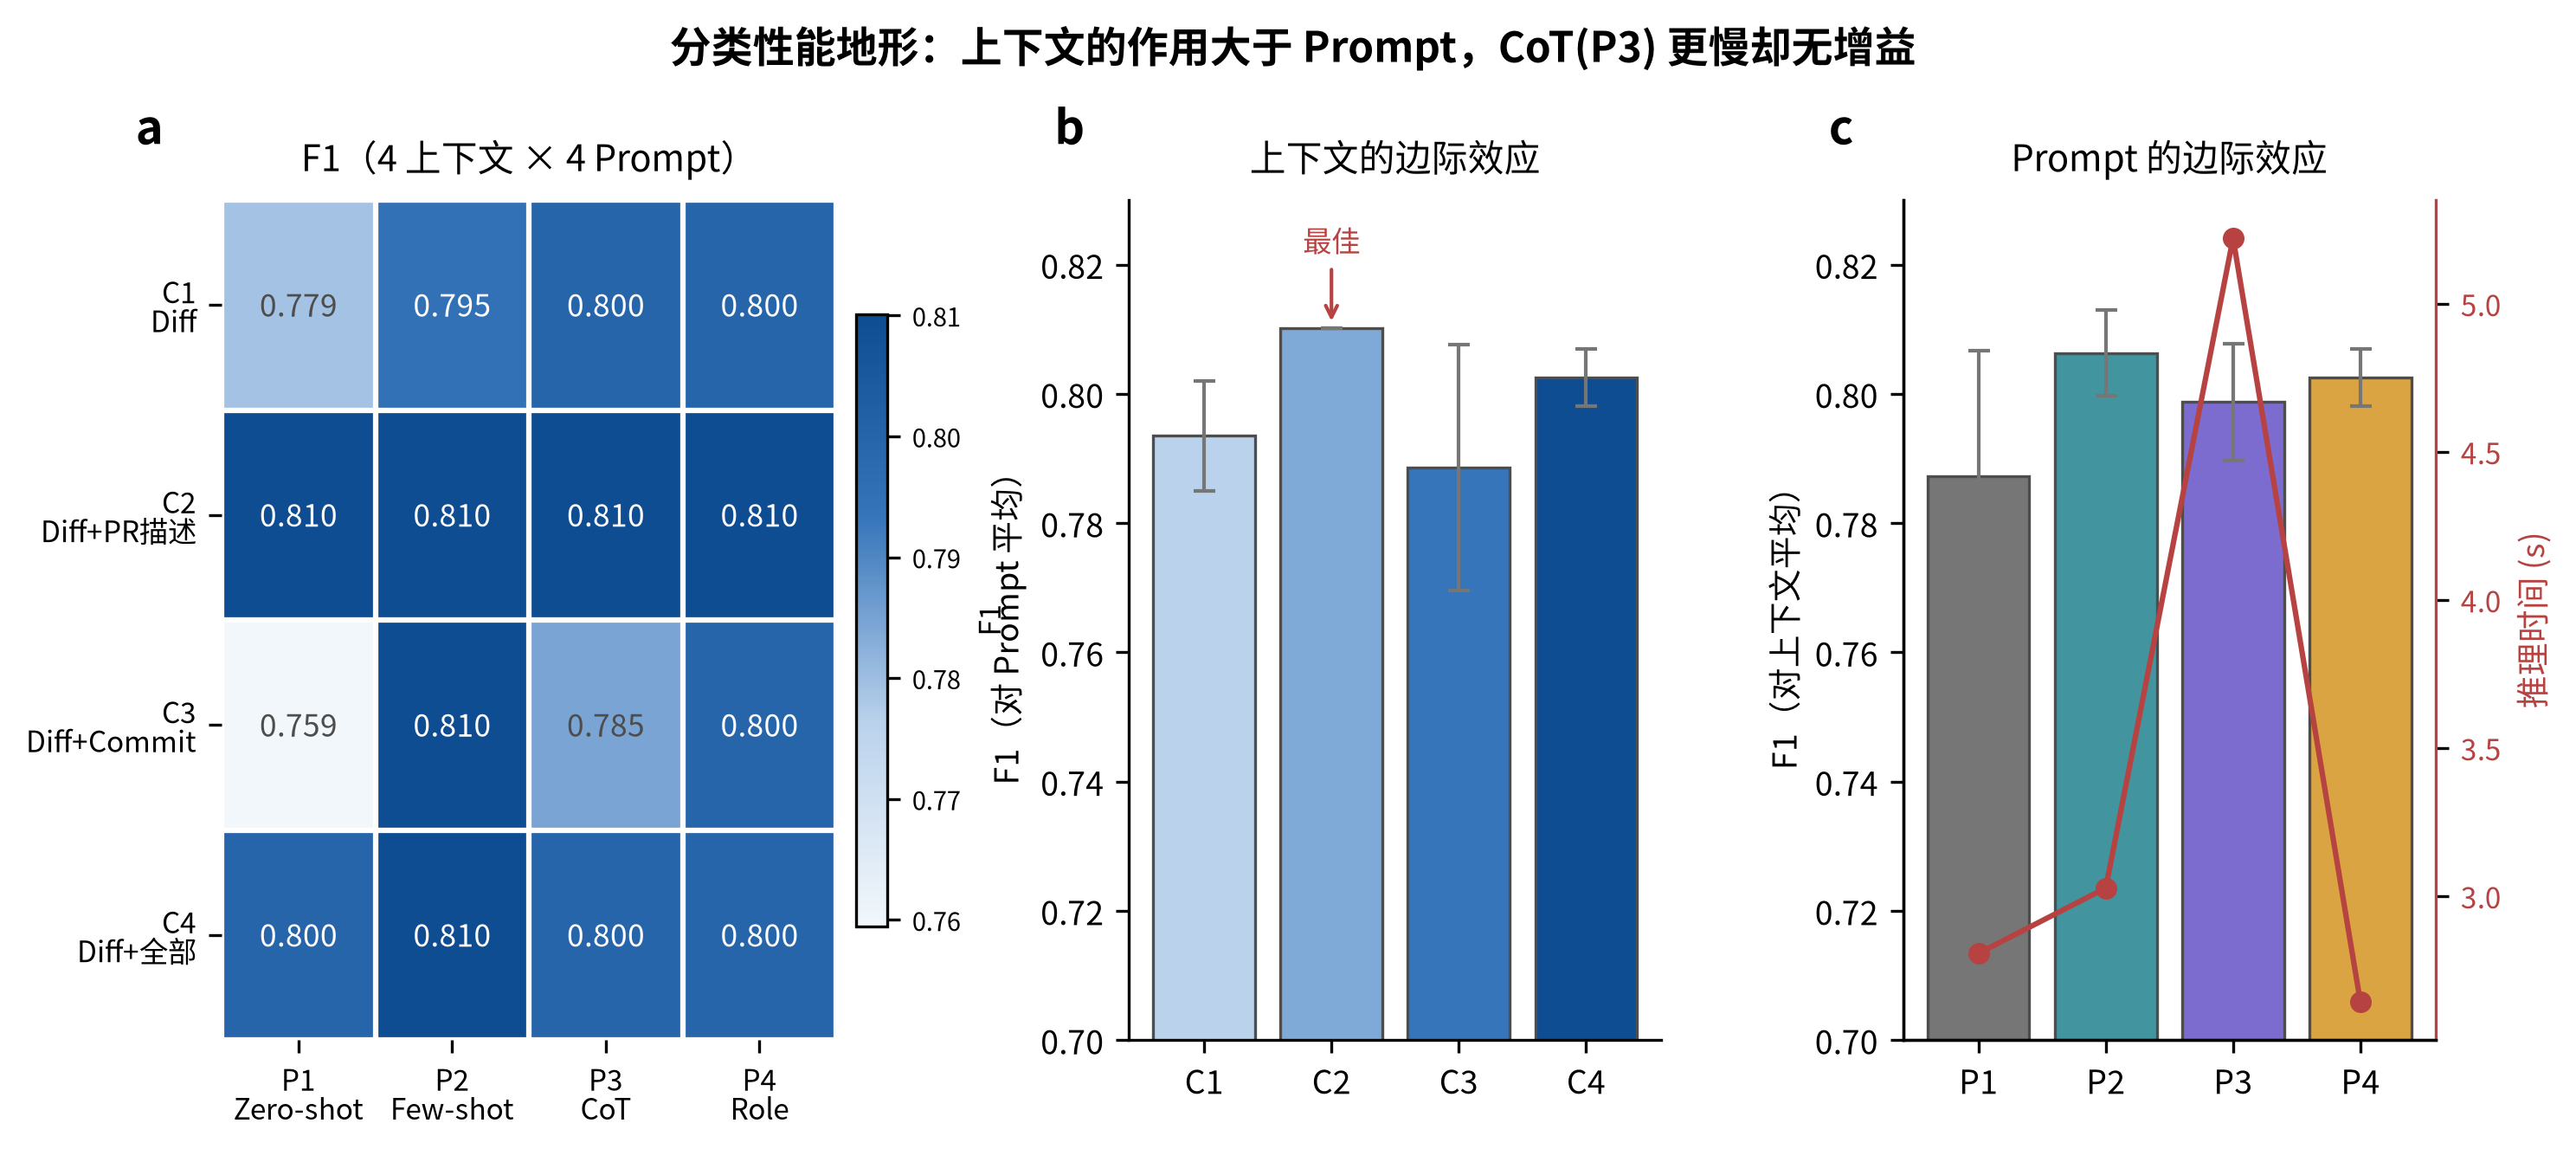
\includegraphics[width=\textwidth]{fig1_classify_landscape.png}
\caption{\textbf{分类性能地形。}（a）16 条件的 F1 热力图（行$=$上下文，列$=$Prompt）；（b）上下文的边际效应（对 Prompt 取均值，误差棒为标准差），C2 最高、C3 最低；（c）Prompt 的边际效应（对上下文取均值），红色折线（右轴）为平均推理时间，可见 CoT(P3) 显著更慢。}
\label{fig:classify}
\end{figure}

从数值上看，全部 16 个条件的 F1 落在 0.759--0.810 的窄带内，最优 F1 为 0.810、最高 Accuracy 仅 0.70。沿上下文方向（图~\ref{fig:classify}b），C2（Diff$+$PR 描述）在四个 Prompt 上一致取得最优 F1（0.810），而 C3（Diff$+$Commit）反而最弱，其 C3\_P1 的 F1 仅 0.759、Accuracy 掉到 0.62；沿 Prompt 方向（图~\ref{fig:classify}c），四种策略的边际差异更小，其中 Few-shot（P2）略稳，而 CoT（P3）不仅没有增益，平均推理时间还从约 2.7~s 抬升到 4--7~s。由此可得两点结论：其一，在合并预测上，改变喂入的上下文比改变提示策略更能撬动性能；其二，更多上下文并不等于更好——加入 PR 描述（C2）带来一致的小幅增益，但叠加 commit message（C3）反而引入噪声、拖低判定。这与任务直觉吻合，PR 描述承载为什么改的意图、缩小了模型的歧义空间，而 commit message 多为琐碎的过程记录，稀释了关键信号；CoT 则在这类一句话判定任务上属于过度推理，只增延迟不增质量。

\subsection*{3.2 失效模式与跨范式对比}

上一节窄带 F1 的表象掩盖了一个更深的问题：模型究竟\emph{凭什么}拿到这样的 F1。为回答这一问题，我们拆解了 16 个条件的精确率—召回率结构，让实验二的 4 个传统 ML 模型在同一 50 条子集上重新预测作对照，并统计每个条件真正识别出应被拒绝的 PR的数量（图~\ref{fig:failure}），参照零点则取全判 MERGE的基线 Accuracy 0.64（子集中 32/50 为 merged）。

\begin{figure}[H]
\centering
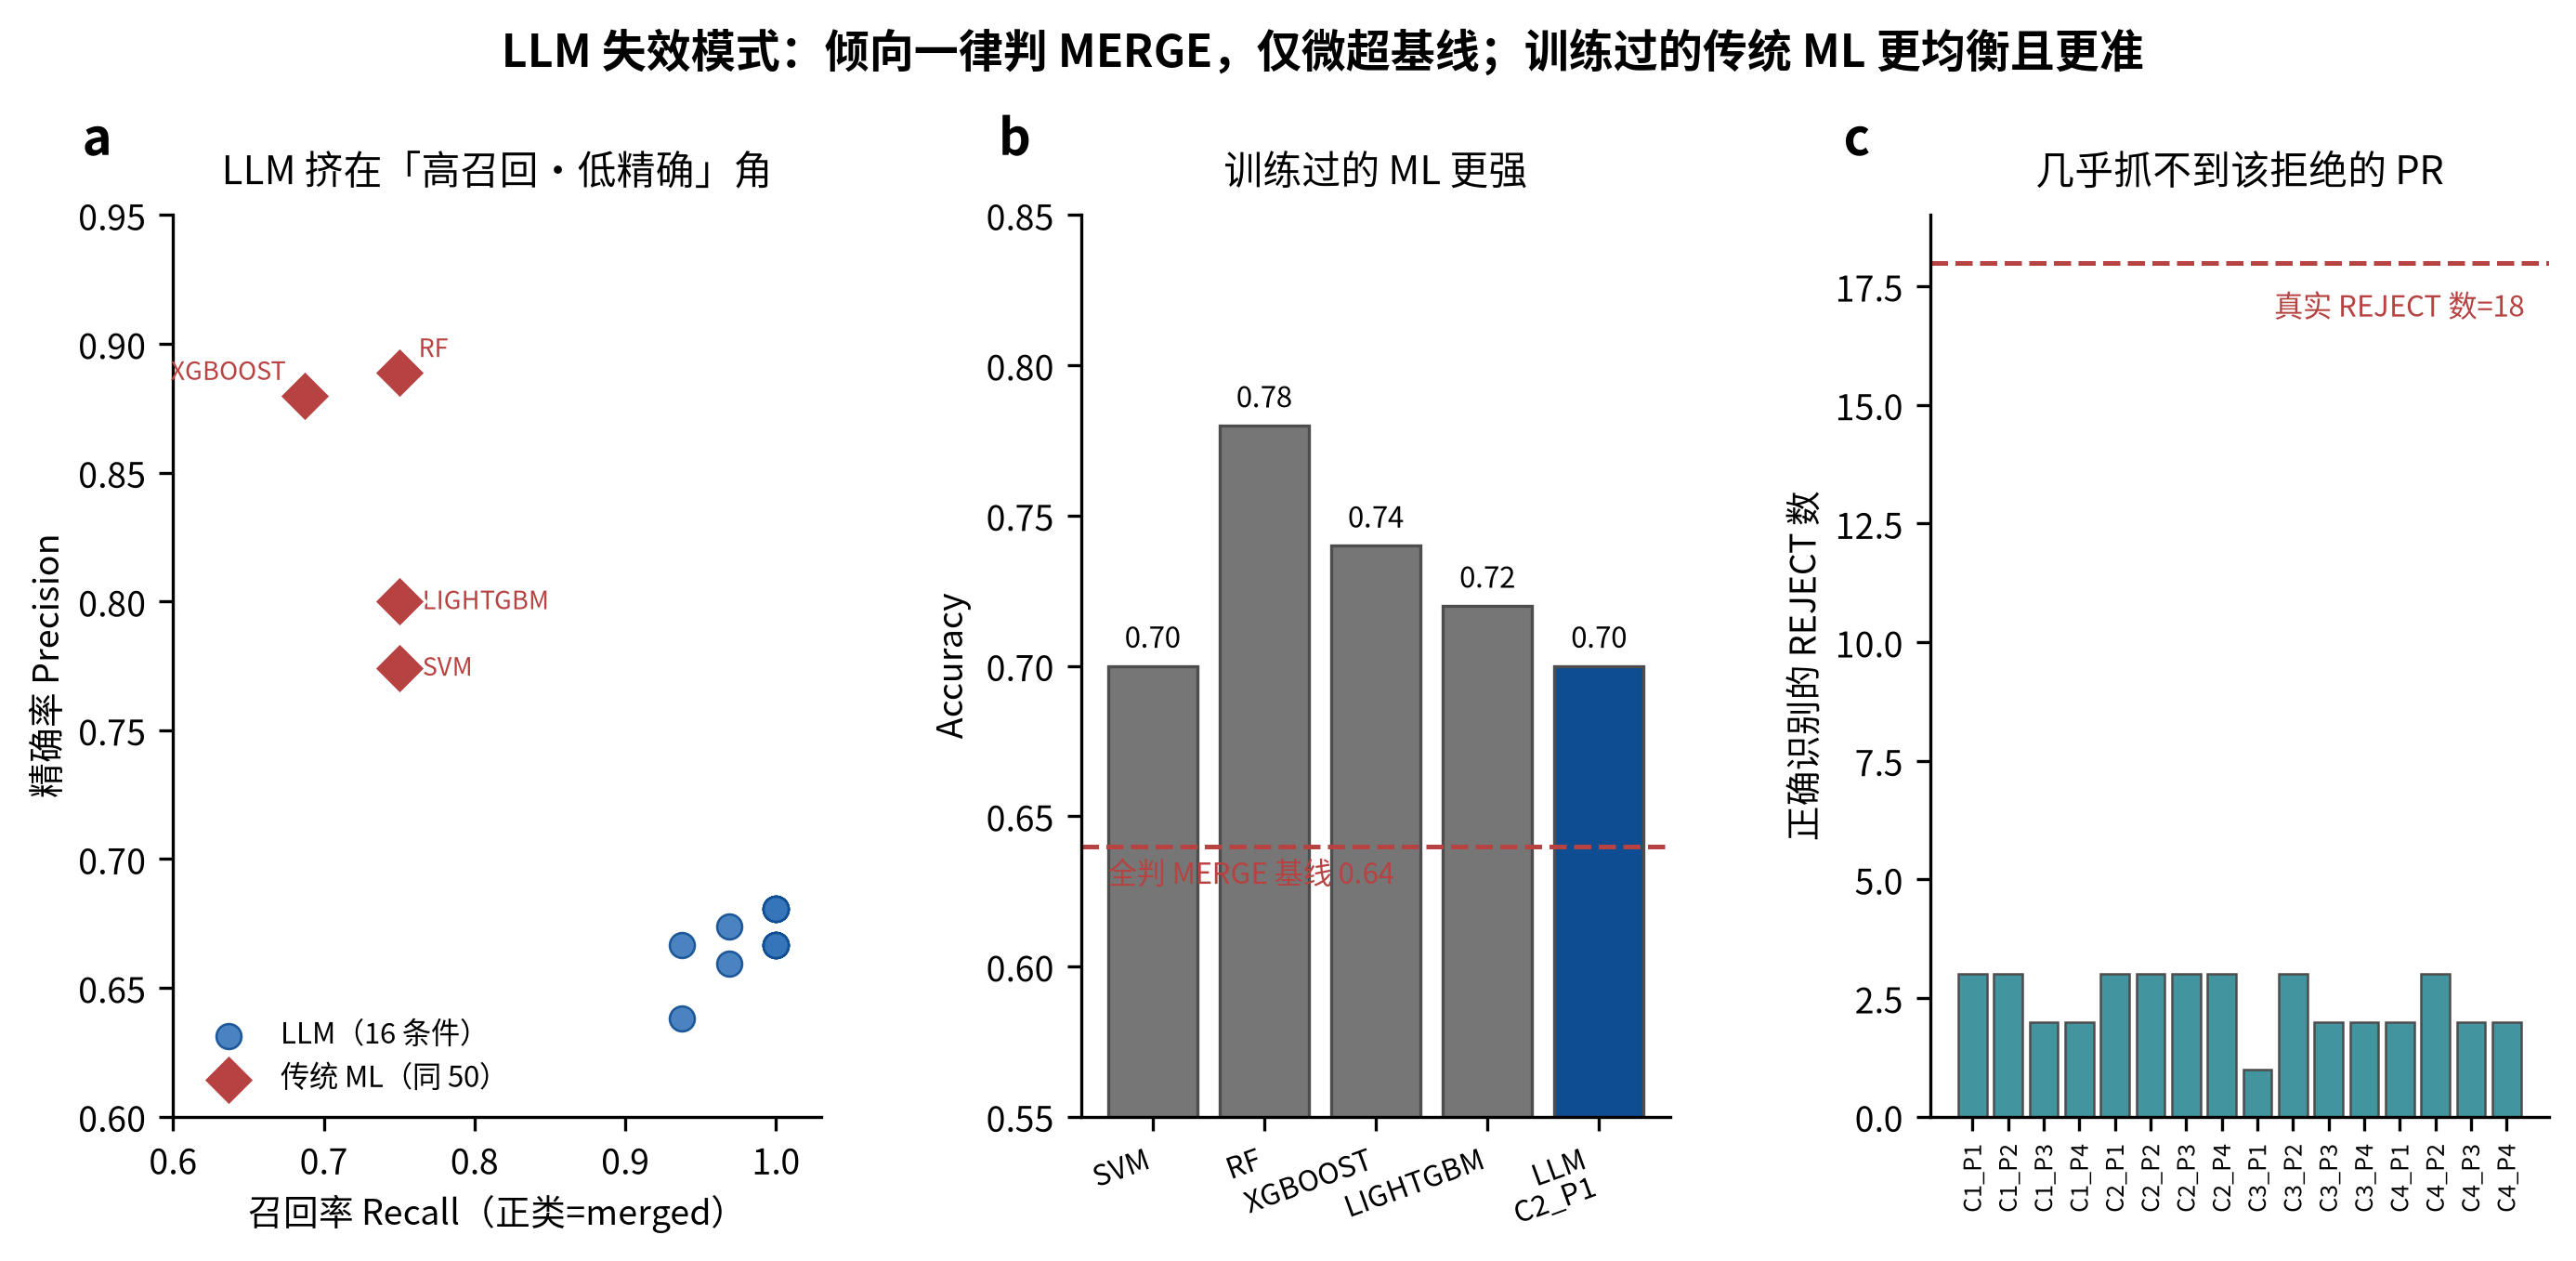
\includegraphics[width=\textwidth]{fig2_llm_failure.png}
\caption{\textbf{LLM 失效模式与同集 ML 对比。}（a）精确率—召回率散点：16 个 LLM 条件（蓝点）挤在高召回、低精确角，4 个 ML 模型（红菱）更均衡；（b）Accuracy 对比，红色虚线为全判 MERGE基线 $0.64$，最佳 LLM 条件仅微超基线，而 RF 达 $0.78$；（c）各条件正确识别出的 REJECT 数，红线为真实 REJECT 总数（18），所有条件都远低于该线。}
\label{fig:failure}
\end{figure}

三个面板指向同一现象。图~\ref{fig:failure}a 中，16 个 LLM 条件几乎全部落在召回率约 1.0、精确率约 0.66--0.68 的角落，即模型近乎无差别地把 PR 判为 MERGE；其直接后果见图~\ref{fig:failure}c，18 条真实应拒绝的 PR 中，绝大多数条件只能正确识别 0--2 条。对照之下，训练过的 ML 更均衡（图~\ref{fig:failure}a 中红菱分布在中部），随机森林的 Accuracy 达 0.78、F1 达 0.814（Precision 0.889、Recall 0.75），而最佳 LLM 条件的 Accuracy 0.70 仅比基线 0.64 高出 0.06（图~\ref{fig:failure}b）。据此可以得出结论：LLM 看似体面的 F1 实则源于一种退化策略——几乎一律判 MERGE，在合并基率本就偏高（0.64）的数据上，这种策略天然拿到高召回与不难看的 F1，却几乎丧失了代码审查最关键的能力，即挑出有问题、该被拒绝的改动。免训练 LLM 在此任务上仅微超多数类基线，而在训练数据上学过判定尺度的轻量 ML 模型（尤以 RF 为最）更均衡、也更准。这表明对于有明确标签与特征的判定任务，训练一个小模型仍显著优于零训练的通用 LLM，与实验二、三专用模型在判别任务上更可靠的发现一脉相承，也为实验七的部署选型提供了直接依据。

\subsection*{3.3 审查意见生成：任务本质困难，富上下文无稳定增益}

审查意见生成的评测方法是对 16 个条件计算语料级 BLEU-4 与 ROUGE-L（完整数值见表~\ref{tab:generate}），并把预测意见与人类意见的字符长度分布对照绘出（图~\ref{fig:generate}）。

\begin{table}[H]
\centering
\caption{审查意见生成 16 条件指标（$N=50$）。BLEU 为语料级 BLEU-4，ROUGE 为 F-measure。}
\label{tab:generate}
\small
\begin{tabular}{l cccc c}
\toprule
条件 & BLEU & ROUGE-1 & ROUGE-2 & ROUGE-L & 推理时间 (s) \\
\midrule
C1\_P1 & \textbf{1.31} & 0.064 & 0.011 & 0.052 & 10.96 \\
C1\_P2 & 1.22 & 0.051 & 0.009 & 0.043 & 11.08 \\
C1\_P3 & 1.25 & 0.058 & 0.008 & 0.052 & 17.20 \\
C1\_P4 & 0.98 & 0.046 & 0.013 & 0.041 & 8.99 \\
C2\_P1 & 1.16 & 0.058 & 0.011 & 0.045 & 9.22 \\
C2\_P2 & 1.15 & 0.057 & 0.010 & 0.051 & 10.36 \\
C2\_P3 & 0.75 & 0.043 & 0.008 & 0.039 & 16.38 \\
C2\_P4 & 1.07 & 0.043 & 0.010 & 0.037 & 9.29 \\
C3\_P1 & 0.66 & 0.049 & \textbf{0.015} & 0.038 & 11.87 \\
C3\_P2 & 0.52 & 0.036 & 0.006 & 0.030 & 11.78 \\
C3\_P3 & 0.87 & 0.055 & 0.010 & 0.046 & 15.37 \\
C3\_P4 & 0.96 & 0.050 & 0.012 & 0.042 & 7.20 \\
C4\_P1 & 0.92 & 0.060 & 0.011 & 0.052 & 10.12 \\
C4\_P2 & 0.97 & 0.046 & 0.011 & 0.038 & 11.95 \\
C4\_P3 & 0.67 & 0.041 & 0.007 & 0.036 & 21.42 \\
C4\_P4 & 0.96 & 0.046 & 0.012 & 0.041 & 8.86 \\
\bottomrule
\end{tabular}
\end{table}

\begin{figure}[H]
\centering
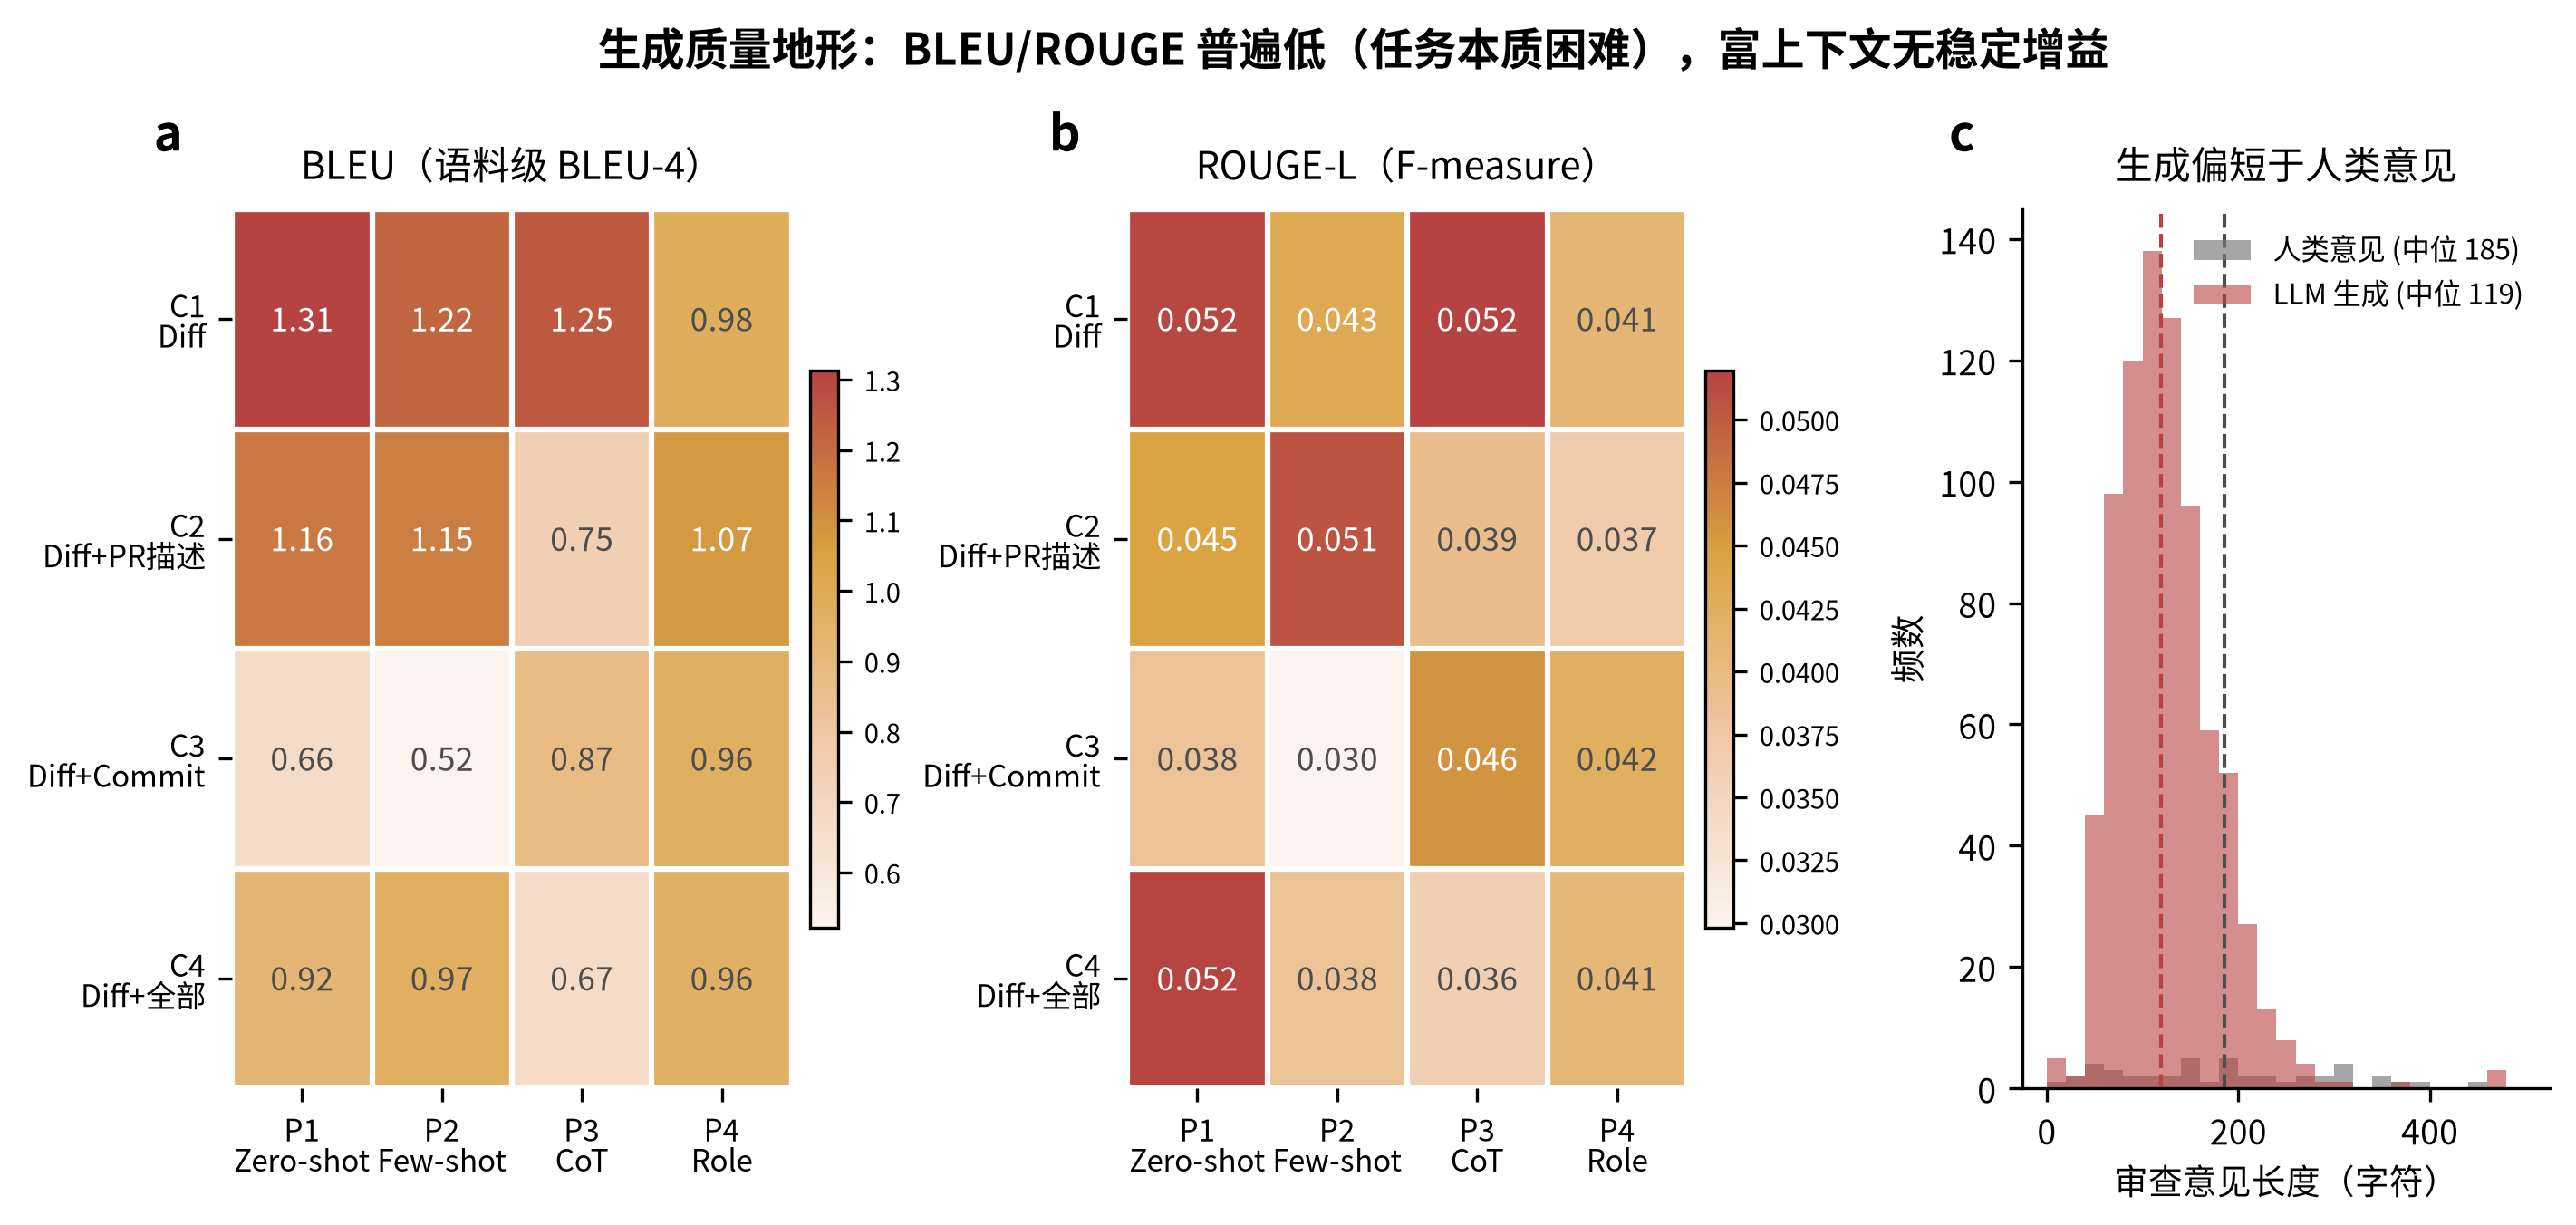
\includegraphics[width=\textwidth]{fig3_generate_landscape.png}
\caption{\textbf{生成质量地形。}（a）BLEU 热力图；（b）ROUGE-L 热力图；（c）预测意见（红）与人类意见（灰）的字符长度分布，虚线为各自中位数，LLM 生成整体偏短。}
\label{fig:generate}
\end{figure}

全部条件的 BLEU 落在 $0.52$--$1.31$、ROUGE-L 落在 $0.030$--$0.052$ 的极低区间，无一条件例外。与分类相反，这里最朴素的 C1\_P1（仅 Diff $+$ Zero-shot）反而取得最高 BLEU（$1.31$），而叠加 commit（C3）或启用 CoT（P3）多数时反而更低（如 C3\_P2 的 BLEU 仅 $0.52$）；长度分布（图~\ref{fig:generate}c）则显示 LLM 生成的意见整体短于人类意见。这一普遍低分首先反映的是\textbf{任务与指标的本质困难而非模型完全失灵}：审查意见生成本质上是高度开放、一对多的任务，面对同一段改动，人类审查者可能聚焦风格、测试、边界或命名中的任意一点，而 BLEU/ROUGE 这类 n-gram 重叠指标会严厉惩罚合理但措辞不同的意见。更值得注意的是，富上下文与复杂 Prompt 在此都没有带来稳定增益，额外信息更像噪声。这与分类任务C2 最优的结论并不矛盾，反而共同指向同一条判断：上下文的价值高度依赖具体任务，并不存在放之四海皆准的越多越好。

\subsection*{3.4 成本—收益：CoT 是一笔没有回报的推理时间税}

最后，为回答更慢的策略是否更好，我们把每个条件的平均推理时间与其质量指标（分类 F1、生成 BLEU）并置考察（图~\ref{fig:cost}）。

\begin{figure}[H]
\centering
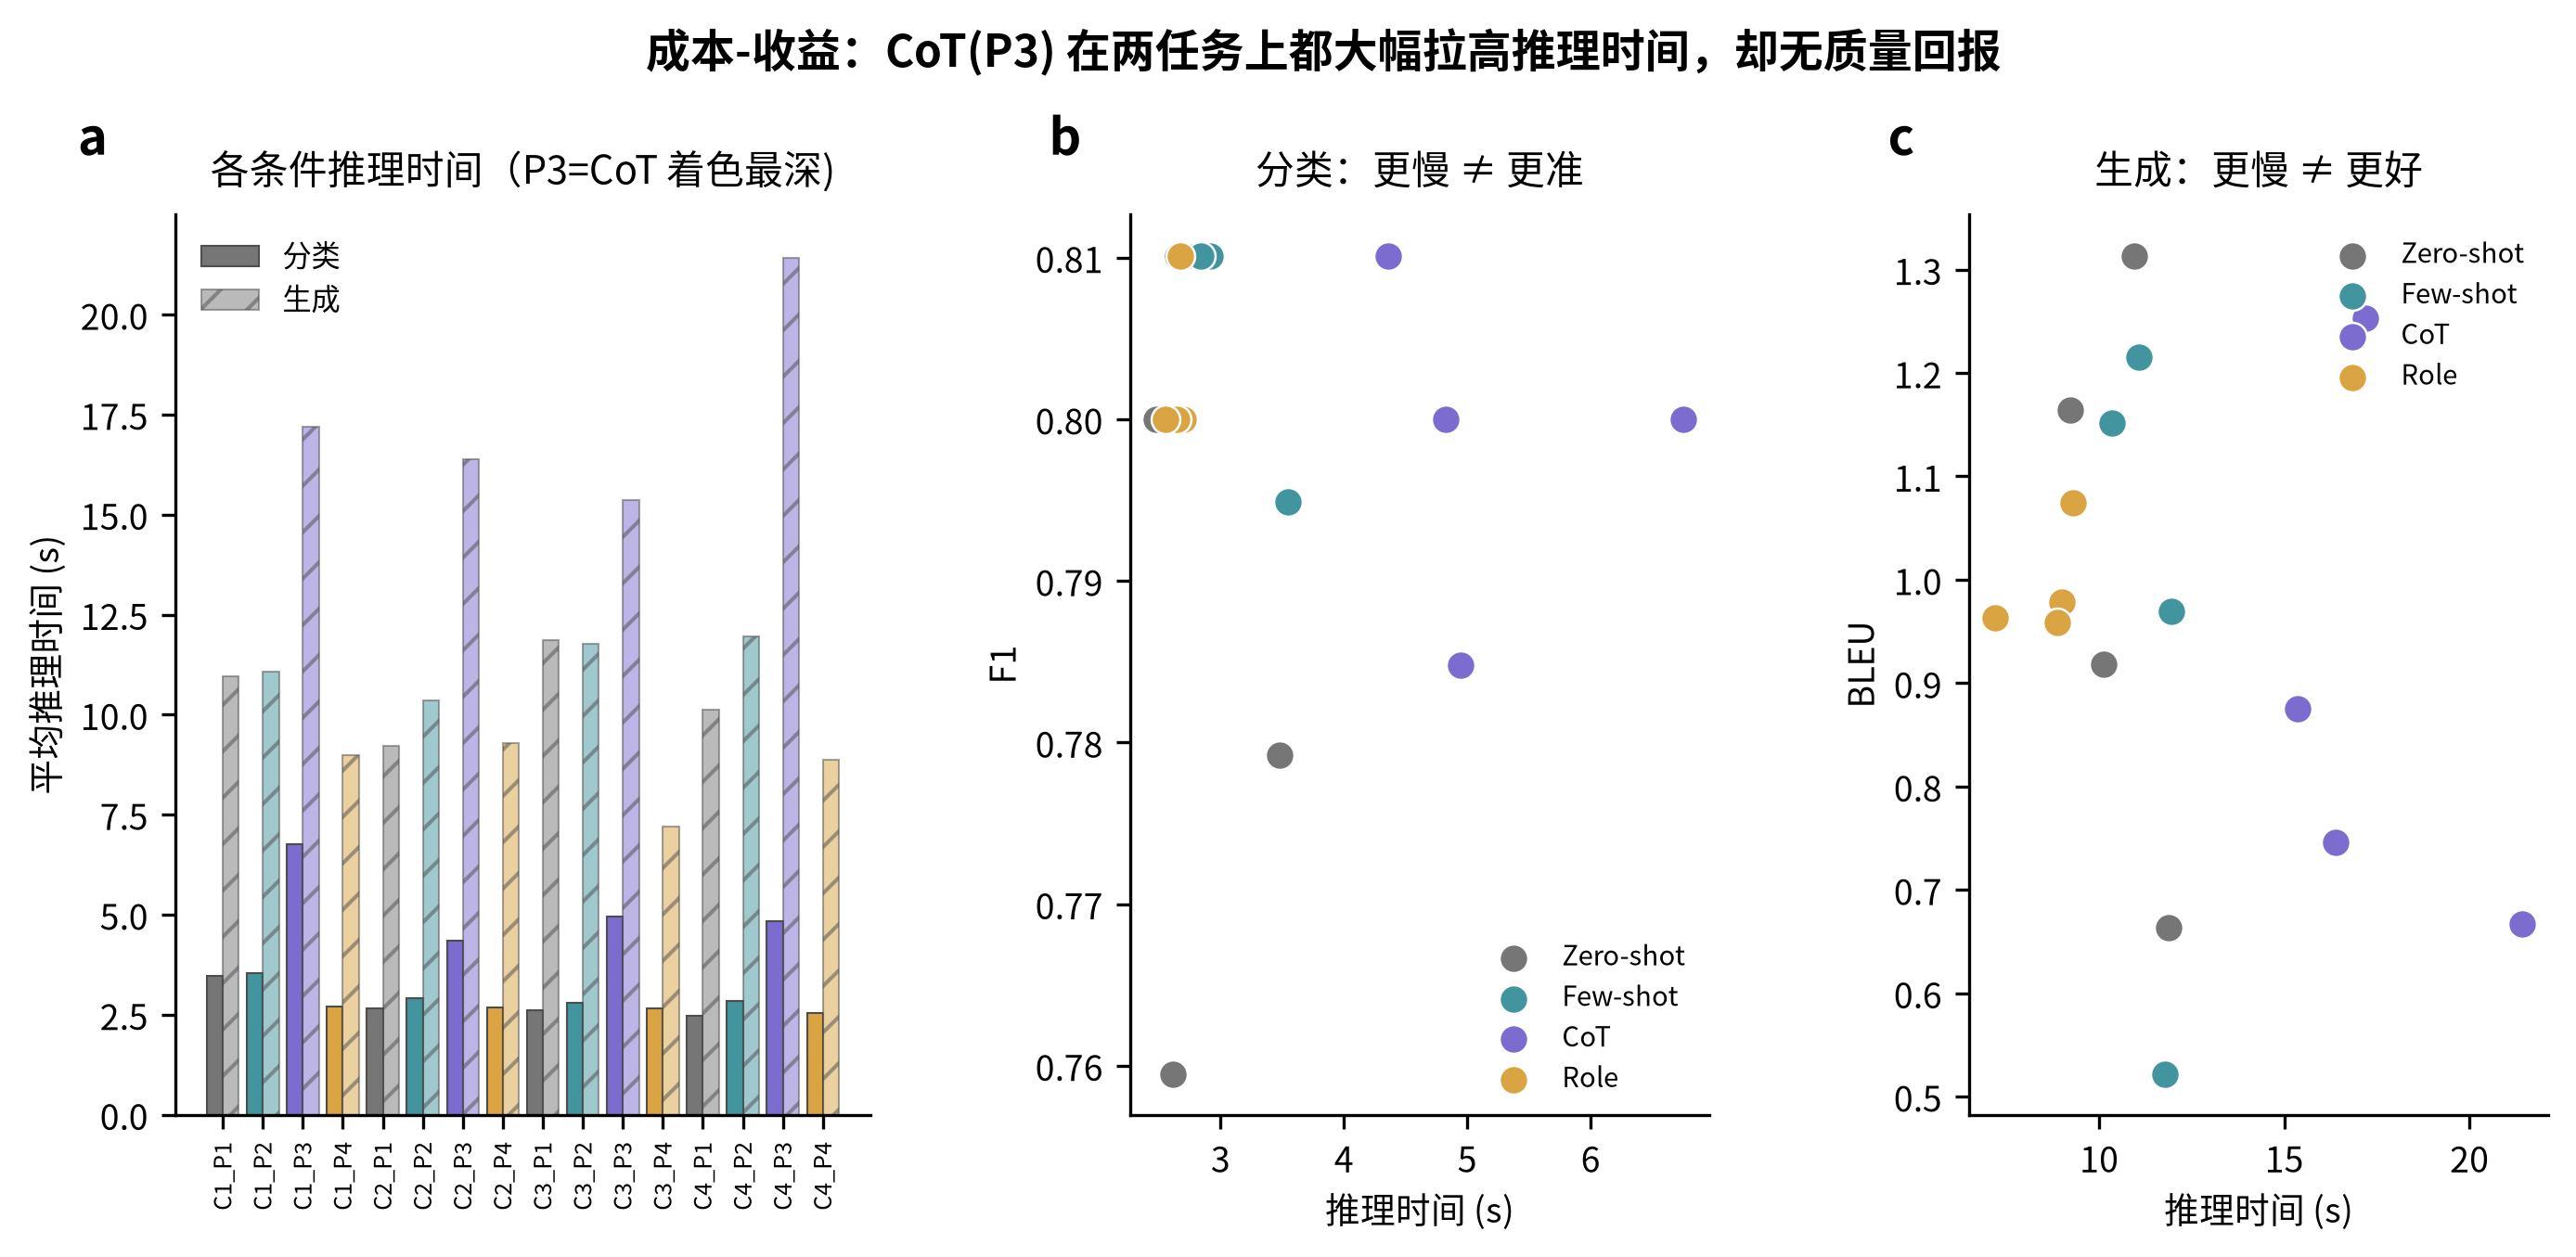
\includegraphics[width=\textwidth]{fig4_latency_cost.png}
\caption{\textbf{成本—收益分析。}（a）各条件平均推理时间（按 Prompt 着色，P3$=$CoT 色最深），CoT 在两任务上都显著更慢；（b）分类：推理时间 vs F1，CoT 点偏右却不偏上；（c）生成：推理时间 vs BLEU，同样更慢 $\neq$ 更好。}
\label{fig:cost}
\end{figure}

可以看到，CoT(P3) 在两个任务上都系统性地拉高延迟——分类从约 $2.7$~s 升到 $4$–$7$~s，生成从约 $9$–$12$~s 升到 $15$–$21$~s（图~\ref{fig:cost}a）；然而图~\ref{fig:cost}b、c 中的 CoT 点只是向右平移（更慢）而非向上抬升（更好），分类 F1 不增，生成 BLEU 甚至多数偏低。由此得出结论：在本实验的两类代码审查任务上，CoT 是一笔几乎没有回报的推理时间税——合并预测是短判定、审查意见生成受 n-gram 指标约束，二者都不吃显式分步推理这一套。这一发现具有直接的工程含义：面向 IDE 内实时审查（实验七）的部署，应优先选择轻量的 Zero-shot 或 Few-shot 配合 C1/C2 上下文，把宝贵的延迟预算留给真正能带来质量回报的环节，而非默认叠加 CoT。

\subsection*{3.5 结果小结}

综合上述四项分析，本实验刻画了一个免训练 LLM 代码审查方案的能力边界与收益结构。在合并预测上，上下文比 Prompt 更能撬动性能，但 C2 最优、C3 反而有害，说明更多上下文并非更好；进一步的失效模式分析显示，LLM 退化为近乎一律判 MERGE，仅微超多数类基线，被训练过的 RF 明显超越。在审查意见生成上，受任务本质与 n-gram 指标的双重约束，各条件普遍低分，且富上下文与复杂 Prompt 均无稳定增益。贯穿两个任务的成本—收益分析则表明 CoT 只增延迟不增质量。这些结论共同回答了本实验的核心问题：在冻结模型的前提下，输入设计确实能调制审查质量，但其收益高度依赖具体任务，且尚未追平训练一个针对性小模型的收益——这既界定了 LLM 的适用场景，也为后续实验六的多粒度上下文增强与实验七的插件选型提供了清晰参照。

}

%========================
% 问题总结
%========================

\experimentproblems{

\subsection*{4.1 在线调用的稳定性与可复现性}

本实验共包含 1{,}600 次在线 LLM 调用。若直接顺序调用，一次网络异常、限流或中断都会影响整轮实验，并可能在重跑时重复计费。为此，将所有请求收拢到 \texttt{llm\_client.py}：同时以任务、上下文、Prompt 和 PR 标识构造语义缓存键，这样，已经完成的条件可以直接复用，中断后能够从未完成的调用继续执行，也使结果分析能够追溯到对应的模型输出。

\subsection*{4.2 上下文长度与对照公平性}

一个 PR 可能包含多个文件和较长的 patch，若无约束地拼接 diff、描述和 commit message，C4 等富上下文条件不仅输入更长，也会让上下文类型与输入长度混在一起，难以公平比较。对此，本实验优先保留 diff，并为 diff、PR body 和 commit message 分别设置约 6{,}000 token、4{,}000 字符和 3{,}000 字符的预算；超出部分显式截断。该处理保证四种上下文在可控的预算内逐步增加改动意图信息，也避免将更多文本误当作更有效的上下文。

\subsection*{4.3 输出解析与生成指标的解释}

LLM 的自由文本输出若无法稳定解析，会给分类和生成指标引入额外噪声。因此，两个任务均使用 JSON 模式：分类读取 \texttt{reasoning} 与 \texttt{decision} 字段，生成读取 \texttt{comment} 字段；解析时先尝试 JSON，再以正则表达式兜底，分类解析失败时额外重试一次。最终 16 个分类条件的解析弃权率均为 0。另一方面，审查意见生成的 BLEU/ROUGE 普遍较低，不能简单等同于模型没有产生有效意见：同一改动可能对应多种合理的审查关注点，而本实验每个 PR 仅以一条人工意见作参照。因此，后续分析将这些指标用于条件间的相对比较，并结合生成长度分布解释，而不将其视为唯一的质量标准。

}

%========================
% 实验体会
%========================

\experimentexperience{

\subsection*{5.1 对上下文与 Prompt 作用的认识}

本实验表明，大语言模型的效果并不只由模型本身决定，输入中提供什么信息同样重要。对于 Merge Prediction，加入 PR 描述的 C2 在四种 Prompt 下均取得最高 F1（0.810），而加入 commit message 的 C3 并未稳定提升，说明与改动意图直接相关的信息比简单堆叠文本更有价值。Prompt 的边际差异则较小，进一步说明上下文设计和 Prompt 设计应结合具体任务验证，不能假定更复杂的策略一定更好。

\subsection*{5.2 对评估协议的认识}

本实验也加深了对指标解释的认识。LLM 在合并预测中的 F1 最高可达 0.810，但进一步拆解后发现其大量预测为 MERGE，只比全判 MERGE 的 Accuracy 基线 0.64 略高；同一子集上的随机森林 Accuracy 为 0.78，分类行为更均衡。因此，评价代码审查模型时不能只看单一 F1，还应结合类别基率、Precision--Recall 结构、错误类型和同集基线。对于审查意见生成，BLEU/ROUGE 的低重叠也提示需要区分“措辞不一致”和“意见无价值”这两类情况。

\subsection*{5.3 对工程部署的认识}

大语言模型的优势在于免训练、能够快速替换上下文和 Prompt；其代价则是在线调用延迟、成本以及输出稳定性。实验中 CoT 在两个任务上都显著增加推理时间，却没有带来稳定质量增益。因而，面向后续实验和 IDE 内实时审查，较合适的策略是在轻量 Zero-shot 或 Few-shot 与 C1/C2 上下文之间进行选择，并把训练过的传统模型作为合并预测的重要基线。整体来看，本实验不仅比较了不同提示策略，也明确了 LLM 在代码审查任务中的适用边界。

}

%========================
% 教师评语
%========================

\teachercomment

\end{document}
